
\chapter{绪论}\label{ch_intro}

\section{本章概要}

\paragraph{一句话描述}

用”hello world“程序作为向导,站在一万米的高空看操作系统的发展和特征!

\paragraph{概述}

计算机系统是由硬件和系统软件((主要是操作系统)组成的,它们共同工作来运行应用程序。纵观计算机相对很短的发展史,虽然计算机系统的具体实现方式不断变化,越来越复杂,但是计算机系统内在的概念保持相对稳定。所有计算机系统在原理上基于天才的图灵机,在设计上基于伟大的冯诺依曼架构,有相似的硬件和软件组件,它们执行着相似的功能。本章主要以操作系统为主来理解计算机系统如何支持一个C语言编写的”hello world“程序完成它的功能。

这里先简要介绍一下操作系统的历史,然后将从一个C语言编写的”hello world“程序开始,讲述操作系统和涉及到的编译,计算机原理等的一些基础知识,以及对操作系统的基本架构和用于本书的ucore教学操作系统做一个初步介绍。在其中穿插介绍操作系统的基本概念、操作系统抽象以及操作系统的特征。

%
%本书希望通过设计实现操作系统来更好地理解操作系统原理和概念。设计实现操作系统其实就是设计实现一个可以管理CPU、内存和各种外设,并管理和服务应用软件的系统软件。为此还是需要先了解一些基本的计算机原理和编程的知识。本书的例子和描述需要读者学习过计算机原理课程、程序设计课程,掌握C语言编程(了解指针等的编程)。如需完成基于RISCore实验,则对基于RISC-V的体系结构有一定的了解,大致了解RISC-V的汇编语言。

%\section{预备知识}
本书希望通过设计实现操作系统来更好地理解操作系统原理和概念。设计实现操作系统其实就是设计实现一个可以管理CPU、内存和各种外设,并管理和服务应用软件的系统软件。为此还是需要先了解一些基本的计算机原理和编程的知识。本书的例子和描述需要读者学习过计算机原理课程、程序设计课程,掌握C语言编程(了解指针等的编程)。如需完成基于RISC-V的ucore实验,则对基于RISC-V的体系结构有一定的了解,大致了解RISC-V的汇编语言。

\section{初步了解操作系统}

我们可以把软件分成应用软件和系统软件。所谓应用软件,即完成某种特定应用功能的软件,比如写文档的office软件,玩游戏的游戏软件等。所谓系统软件,即完成系统功能的软件,这里的系统功能相对与特定应用功能而言,更加底层和通用,比如编译器,C运行时库,操作系统等。而对于系统软件,我们又可以分为系统应用((编译器,C运行时库等)和操作系统。这里把操作系统单独分出来,是由于操作系统直接管理了硬件,所有的应用都需要操作系统的支持,才能正常工作。

操作系统其实是一个相比较复杂的系统软件,直接管理计算机硬件和各种外设,以及给应用软件提供帮助。这样描述还太简单了一些,我们可对其进一步描述:操作系统是一个可以管理CPU、内存和各种外设,并管理和服务应用软件的软件。为了完成这些工作,操作系统需要知道如何与硬件打交道,如何更好地服务好应用软件。

\subsection{操作系统历史}

在大众的眼中,操作系统就是他们的手机/终端上的软件系统,包括各种应用程序集合,但在历史上,操作系统也是从无到有地逐步发展起来的。操作系统主要完成对硬件控制和对应用程序的服务所必需的功能,操作系统的历史与计算机发展的历史密不可分。操作系统的内涵和功能随着历史的发展也在一直变化,改进中,在今天,没有图形界面和各种文件浏览器已经不能称为一个操作系统了。

\subsubsection{三叶虫时代}

计算机在最开始出现的时候是没有操作系统的。启动,扳开关,装卡片/纸带等比较辛苦的工作都是计算机操作员(Operator)或者用户自己完成。操作员/用户带着记录有程序和数据的卡片(punch card)或打孔纸带去操作机器。装好卡片/纸带后,启动卡片/纸带阅读器,让计算机把程序和数据读入计算机机的内存中后,计算机就开始工作,并把结果也输出到卡片/纸带或显示屏上,最后程序停止。

由于人的操作效率太低,计算机的机时宝贵,所以就引入监控程序(Monitor)辅助完成输入,输出,加载,运行程序等工作,这是现代操作系统的起源。一般情况下,计算机每次只能执行一个任务,CPU大部分时间都在等待人的缓慢操作。

\subsubsection{恐龙时代}

早期的操作系统非常多样化,专用化,生产商生产出针对各自硬件的专用操作系统,大部分用汇编语言编写,这导致操作系统的进化比较缓慢,但进化再持续。在1964年,IBM公司开发了面向System/360系列机器的统一可兼容的操作系统——OS/360。OS/360是一种批处理操作系统。为了能充分地利用计算机系统,应尽量使该系统连续运行,减少空闲时间,所以批处理操作系统把一批作业(古老的术语,可理解为现在的程序)以脱机方式输入到磁带上,并使这批作业能一个接一个地连续处理:1)将磁带上的一个作业装入内存;2)并把运行控制权交给该作业;3)当该作业处理完成后,把控制权交还给操作系统;4)重复1-3的步骤。

批处理操作系统分为单道批处理系统和多道批处理系统。单道批处理操作系统只能管理内存中的一个(道)作业,无法充分利用计算机系统中的所有资源,致使系统整体性能较差。多道批处理操作系统能管理内存中的多个(道)作业,可比较充分地利用计算机系统中的所有资源,提升系统整体性能。二者的共同特点是人机交互性差,这对修改和调试程序很不方便。

\subsubsection{爬行动物时代}

20世纪60年代末,提高人机交互方式的分时操作系统越来越展露头角。分时是指多个用户和多个程序以很小的时间间隔来共享使用同一台计算机上的CPU和其他硬件/软件资源。1964年由贝尔实验室、麻省理工学院及美国通用电气公司所共同参与研发目标远大的MULTICS(MULTiplexed Information and Computing System)操作系统,MULTICS是一套安装在大型主机上多人多任务的操作系统。 MULTICS以兼容分时系统(CTSS)做基础,建置在美国通用电力公司的大型机GE-645,目标是连接1000部终端机,支持300的用户同时上线。因MULTICS项目的工作进度过于缓慢,1969年AT\&T的 Bell 实验室从MULTICS 研发中撤出。但贝尔实验室的两位软件工程师 Thompson 与 Ritchie借鉴了一些重要的Multics理念,以C语言为基础,发展出UNIX操作操作系统。UNIX操作系统的早期版本是完全免费的,可以轻易获得并随意修改,所以它得到了广泛的接受。后来,它成为开发小型机操作系统的起点。由于早期的广泛应用,它已经成为的分时操作系统的典范。

\subsubsection{哺乳动物时代}

20世纪70年代,微型处理器的发展使计算机的应用普及至中小企及个人爱好者,推动了个人计算机(Personal Computer)的发展,也进一步推动了面向个人使用的操作系统的出现。其代表是由微软公司中在20世纪80年代为个人计算机开发的DOS/Windows操作系统,其特点是简单易用,特别是基于Windwos操作系统的GUI界面,极大地简化了一般用户使用计算机的难度,使得计算机得到了快速的普及。这里需要注意的是,第一个带GUI界面的个人计算机原型起源于伟大却又让人扼腕叹息的施乐帕洛阿图研究中心PARC(Palo Alto Research Center),PARC研发出的带有图标、弹出式菜单和重叠窗口的GUI(Graphical User Interface),可利用鼠标的点击动作来进行操控,这是当今我们所使用的GUI系统的基础。

\subsubsection{智人时代}

21世纪以来,Internt和移动互联网的迅猛发展,使得在服务器领域和个人终端的应用与需求大增。iOS和Android操作系统是21世纪个人终端操作系统的代表,Linux在巨型机到数据中心服务器操作系统中占据了统治地位。以Android系统为例,Android一词英文本义指“机器人”,它是由Google公司于2007年11月推出的基于Linux Kernel的开源手机操作系统,目前在移动终端中占有最大的份额。Android操作系统是一个包括Linux操作系统内核、基于Java的中间件、用户界面和关键应用软件的移动设备软件栈集合。这里介绍一下广泛用在服务器领域和个人终端中的操作系统内核--Linux操作系统内核。1991年8 月,芬兰学生 Linus Torvalds(林纳斯·托瓦兹)在 comp.os.minix 新闻组贴上了以下这段话: 

"你好,所有使用 minix 的人 -我正在为 386 ( 486 ) AT 做一个免费的操作系统 ( 只是为了爱好 ),不会像 GNU 那样很大很专业。″

而他所说的"爱好″就变成我们今天知道的 Linux操作系统内核。 Linus通过Internet首次发表 Linux kernel的源代码,并且选用GPL版权协议来发行。GPL版权协议允许任何人以任何形式发布 Linux 的源代码,在Internet的日渐盛行以及 Linux 开放自由的GPL版权之下,吸引了无数计算机Hacker和公司投入开发、改善 Linux kernel,使得 Linux kernel的功能日见强大。 

\subsubsection{神人时代}

当前,大数据、人工智能、机器学习、高速网络、AR/VR对操作系统等系统软件带来了新的挑战。如何有效支持和利用这些技术是未来操作系统的方向。



\subsection{hello world漫游}

本节希望通过显示“hello world!”的应用程序来感受操作系统的功能和特征。一般应用程序都希望能够完成接受输入、显示输出、保存结果、定时处理等基本功能,而这些功能都是在操作系统的帮助下完成的。

\subsubsection{智人时代下的"hello world!"}

智人时代的典型操作系统是Linux和Windows。Linux和Windows都非常强大,在这两个操作系统上编写和执行“显示“hello world!”的各种应用程序很容易,容易到你都感觉不到操作系统的存在。相对而言,Linux可以看到它的源代码,用到的各种工具和操作相对也原始一些,可以让读者与操作系统的距离感更近一些,对于理解操作系统的实现会有很大帮助,所以我们以Linux作为我们的实验环境。
接下来的五个小实验,分别基于不同的需求完成对“hello world!”的显示:
\begin{itemize}
	\item 在显示器上直接显示字符串;
	\item 通过定时器在显示器上定时显示字符串;
	\item 把字符串“显示”到磁盘上永久保存;
	\item 可根据键盘输入改变字符串的显示内容;
	\item 定时显示程序和交互显示程序一起执行。
\end{itemize}

通过这些实验,我们可以看到操作系统的一个重要功能是给应用程序提供了便捷的访问服务,应用程序只需发出要求,比如显示字符串、保存文件、定时唤醒、接收输入等,操作系统就可以帮助它完成;另外还有一些很重要的看不见的管理服务,比如给应用程序提供执行环境,切换应用程序,回收应用程序占用的资源等,这些就不能直接地感受到了。而对于硬件,比如显示器、定时器、磁盘、键盘等各种外设,操作系统都把它们很好地管理起来,提供了外设管理服务,使得我们的应用程序很方便地通过一些简单的AP就可以访问这些外设,而不需要关注外设的复杂控制细节。


\begin{note} 
下面的实验环境是基于ubuntu-16.04 x86-64环境,虽然CPU是x86-64,当下面的实验完全没有涉及到x86-64的细节,所以在这里就直接忽视让操作系统和应用正常运行的这个不可或缺的一个或多个CPU和其他不相关的硬件细节。
\end{note}

\paragraph{显示"hello world!"}
让我们通过智人时代的操作系统Linux来感受一下显示一个字符串的过程。假定读者建立了Linux实验环境(参见\ref{setuplinux}),对C语言有一定的了解,所以可以写出如下的代码 helloworld.c:
\begin{lstlisting}[language={C}]
void main(void)
{
  puts("hello world!");
}
\end{lstlisting}

并在Linux环境中的shell界面下,执行gcc编译命令,把helloworld.c转换成执行程序helloworld:

\begin{lstlisting}[language={bash}]
$ gcc -o helloworld helloworld.c
\end{lstlisting}

在shell界面下,在生成执行程序helloworld的目录下执行此程序,可以看到程序显示出了“hello world!”:
%\begin{lstlisting}[language={bash},numbers=none]
\begin{lstlisting}[language={bash}]
	  $ helloworld
	  hello world!
\end{lstlisting}


只要读者会基本编程,对于上面的输出结果,应该不会感到陌生。但读者对具体的执行过程了解吗?Linux操作系统和它用的x86计算机硬件太复杂,如果要详细分析和解释上面示例的两行显示背后的具体执行过程的细节,我们可以写出一本超过1000页的大部头。考虑到读者时间有限,下面我们将站在操作系统的角度来简单理解一下这个helloworld程序的执行过程。

%上面的操作过程,需要与人交互的有两个外设,一个是键盘,一个是显示器。首先,你看到的是\$符号,这是一个正在运行的程序shell的人机交互界面。在你没敲字符的时候,\textbf{shell处于睡觉状态}。当你通过键盘敲入“g”和后续的多个字符的时候,首先是操作系统收到键盘发出的字符,然后通知shell,有字符来了!shell本来在睡觉,被操作系统唤醒后,接收字符,并发出显示字符的请求给操作系统。操作系统收到shell的请求后,把字符显示到显示器上,然后通知shell完成显示字符任务了。当shell程序收到回车字符的时候,就开始把整个字符串看成是一个命令,解析完此命令后,并告知操作系统,继续请操作系统帮忙执行另外一个程序gcc来完成整个编译过程。操作系统为此需要创建一个让gcc可以正常工作的执行空间,并启动gcc程序,让它能够完成整个编译过程。gcc于是开始干活,首先请操作系统把helloworl操作系统d.c这个文件从磁盘上读到内存中,gcc对内存中的helloworld.c的内容进行编译,生成helloworld执行程序,但此时这个程序还在内存中。于是gcc继续请操作系统帮忙,把这个helloworld执行程序写到磁盘上。当你看到第二个\$符号出现的时候,表示gcc的工作完成了。

%上面的helloworld执行程序需要用到一个个外设:显示器。dang\$上继续敲如字符串"hello world!",并回车。类似上面的描述,这次shell程序会请求操作系统来执行helloworld这个程序。操作系统为此需要创建一个让helloworld程序可以正常工作的执行空间,并启动helloworld程序。helloworld的执行工作就是显示字符串“hello world!”。为此,它像shell一样,给操作系统发出显示字符串的请求。操作系统收到显示字符串的请求后,把字符串显示到屏幕上。至此,上面示例中三行显示的背后执行过程就简单描述完毕。

上面的helloworld执行程序需要用到一个外设:显示器。当你在shell的\$提示符后继续敲如字符串"hello world!"并回车,shell解析此命令,分析出你是要执行helloworld这个程序,于是会请求操作系统来执行helloworld这个程序。操作系统为此需要创建一个让helloworld程序可以正常工作的执行环境(比如分配内存放代码和数据,提供CPU用于执行等),并启动helloworld程序。此时shell程序要让位helloworld程序执行,为此操作系统还要完成一个执行环境切换的过程,让helloworld能够占用CPU来执行。完成切换后,helloworld程序才真正开始执行。

helloworld的执行工作就是显示字符串“hello world!”。为此,它像shell一样,给操作系统发出显示字符串的请求。操作系统收到显示字符串的请求后,直接控制显卡这个设备,通过显卡把字符显示到显示器上,然后通知shell完成显示字符任务了。helloworld程序执行完毕后,操作系统还要把之前分配给helloworld的执行环境给收回,用于其他程序的执行。至此,上面示例中两行行显示的背后执行过程就简单描述完毕。

\begin{note} 
操作系统其实也没有直接控制显示器,而是通过控制显卡,让显卡访问显示器上显示信息的。
\end{note}

\paragraph{每秒定时显示"hello world!"}
如果要每秒定时显示字符串,很显然需要时钟外设来帮助实现定时。添加一点代码形成timing-helloworld.c,就可以实现定时显示helloworld了。
\begin{lstlisting}[language={C}]
void main(void)
{
  while(1) {
    sleep(1);
    puts("hello world!");
  }
}
\end{lstlisting}

在Linux环境中,执行gcc编译命令,把timing-helloworld.c转换成执行程序timing-helloworld,并执行生成的执行程序timing-helloworld:
\begin{lstlisting}[language={bash}]
	$ gcc -o timing-helloworld timing-helloworld.c
	$ timing-helloworld
	hello world!
	hello world!
	......
\end{lstlisting}

可以看到,当执行timing-helloworld程序时,屏幕上会每隔一秒重复显示“helloworld”。新增加的sleep函数完成了等待一秒并恢复执行的功能。其实这个功能也是靠藏在后面的操作系统帮忙完成的。当timing-hellworld执行sleep(1)函数时,它向操作系统发出了一个请求,要求操作系统先让它睡觉,且让操作系统帮它设个1秒到期的闹钟(更正式的说法是定时器)。于是操作系统先把timing-helloworld设置为睡眠状态,且对时钟外设做好配置,让它1秒中后产生一个中断,通知操作系统到点了。操作系统做完这两件事后,就忙自己的其他事情并安排调度其他程序运行。过了1秒后,时钟外设产生了一个中断,通知操作系统到点了,操作系统响应这个中断,并记得timing-hellworld需要被唤醒并继续运行,于是就把timing-hellworld唤醒,并让它继续运行。这样,timing-hellworld就开始每隔1秒显示字符串了。

\paragraph{把"hello world!"字符串存到磁盘上}

如果要把显示字符串长久保存下来,很显然需要磁盘外设来帮助实现长期存储的功能。添加一点代码形成file-helloworld.c,就可以实现把字符串保存到磁盘上了。

\begin{lstlisting}[language={C}]
#include <stdio.h>
void main(void){
  FILE *fp;
  fp = fopen("file-helloworld.txt", "w");
  fputs("hello world!",fp);
  fclose(fp);
}
\end{lstlisting}

在Linux环境中,执行gcc编译命令,把file-helloworld.c转换成执行程序file-helloworld,并执行生成的执行程序file-helloworld:
\begin{lstlisting}[language={bash}]
	$ gcc -o file-helloworld file-helloworld.c
	$ file-helloworld
	$ more file-helloworld.txt
	hello world!	
\end{lstlisting}

可以看到,当执行file-helloworld程序时,当前目录下多了一个文件file-helloworld.txt,通过more命令,可以看到file-helloworld.txt文件的内容就是我们需要保存的字符串"hello world!"。这里我们可以看到通过操作系统,应用程序可用文件的形式方便地把字符串存储到磁盘上,而没有关注磁盘磁盘的细节。当执行程序file-helloworld的时候,操作系统做了啥呢?首先,当file-helloworld执行fopen函数时,会请求操作系统在当前目录下创建一个可写的文件file-helloworld.txt。于是操作系统会定位到当前目录在磁盘上的位置,并在此目录下添加一个文件,此时的文件内容为空。然后当file-helloworld执行fput函数时,会请求操作系统把"hello world!"这个内容写到file-helloworld.txt文件中。于是操作系统定位到file-helloworld.txt文件在磁盘中的位置,给这个文件分配空闲磁盘扇区空间用于存放文件内容,再把位于内存中的字符串"hello world!"以磁盘块为单位,写入到文件内容对应的磁盘扇区中。



\paragraph{交互式显示"hello world!"}

上面三个小实验缺少了一点与人的交互。比如,如果我敲了一个名字“human”,程序就能显示"human, hello world!"。让程序能接收输入,那还需要一个外设:键盘。通过键盘,程序就可以得到人的输入了。getchar-helloworld.c的代码如下:

\begin{lstlisting}[language={C}]
void main(void)
{
  char name[100];
  int i=0;
  while((name[i] = getchar())!='\n' && i<80)
        i++ ;
  name[i]=0;
  strcat(name,", hello world!");
  puts(name);
}
\end{lstlisting}

在Linux环境中,执行gcc编译命令,把getchar-helloworld.c转换成执行程序getchar-helloworld,并执行生成的执行程序getchar-helloworld:
\begin{lstlisting}[language={bash}]
	$ gcc -o getchar-helloworld getchar-helloworld.c
	$ getchar-helloworld
	human
	human, hello world!	
\end{lstlisting}

当执行getchar-helloworld程序时,如果你没敲字符,getchar-helloworld就会默默地等待你的输入\textbf{其实getchar-helloworld处于睡觉状态}。当你通过键盘敲入“h”和后续的多个字符的时候,首先是操作系统收到键盘发出的字符,然后唤醒并通知getchar-helloworld,有字符来了。getchar-helloworld本来在睡觉,被操作系统唤醒后,持续接收字符。在收到'\\n'回车符后,就把用户输入的字符与", hello world!"字符连接在一起,形成一个新字符串,并请求操作系统显示这个新字符串。操作系统接下来的过程与上面的分析解释是一样的,。

\paragraph{定时+交互式显示"hello world!"}
上面的小实验都是执行一个程序,如果把两个执行程序放在一起执行会怎样呢?操作系统会如何管理这两个程序的执行呢?下面我们尝试把上述两个执行程序timing-helloworld和getchar-helloworld放在一起执行:
\begin{lstlisting}[language={bash}]
$ timing-helloworld & getchar-helloworld
[1] 24690
hello world!
hhello world!
uman
human, hello world!
hello world!
...
\end{lstlisting}

上述第一行命令的功能是让timing-helloworld和getchar-helloworld这两个程序都执行。所谓都执行,就是让操作系统来管理这两个程序的执行过程。让输入第一行命令并敲回车键后,shell程序请操作系统帮忙来执行这两个程序。操作系统收到请求后,先创建timing-helloworld程序的执行环境,再创建getchar-helloworld程序的执行环境,然后就开始执行这两个程序了。注意,每次操作系统只能调度一个程序占用CPU执行。在上面小节的分析中,已经描述过了两个程序的单独执行过程,但这里是两个程序一起执行。

当读者进行这个实验时,会碰到类似上面的输出现象,一开始两个程序都会由于等定时器或等用户输入而睡眠,所以操作系统会把两个程序设置为睡眠状态。一秒后,定时器会发出信号,操作系统收到定时器信号后,会唤醒timing-helloworld程序,让它继续显示字符串。在某一时刻,读者开始敲键盘,输入“human”。当输入第一个"h"时,getchar-helloworld程序被操作系统唤醒,并开始接收读者输入的字符。比较奇怪的是第四行的显示“hhello world!”和第五行的“uman”,这其实说明了在getchar-helloworld程序接受用户输入的时候,timing-helloworld程序的下一个一秒到期了,操作系统暂停了getchar-helloworld,切换到timing-helloworld程序继续执行,于是就出现了第四、五行的奇怪输出了。这里总算比较直观地能看到操作系统对多个执行程序执行过程的管理和调度了。

通过上面的五个实验,你会发现程序代码很简单,但默默付出的操作系统做了好多的幕后工作,但这些工作对于执行程序的用户而言都是很难直接看不到的,用户看到的是应用程序shell完成了用户的请求,而幕后英雄--操作系统只是默默的完成应用程序的各种请求。智人时代的操作系统的特点是麻烦自己,方便用户。把自己搞得特别复杂,像Linux kernel这样大家能看到源码的操作系统,其当前最新的4.17版本已经有2千万行代码了。即使是应用程序显示字符串这样一个简单过程,在Linux中执行了的代码行数也都过万行。但这不会影响我们了解其基本原理。

\subsubsection{爬行动物时代下"hello world!"}

虽然通过上面的五个小实验,我们对操作系统的功能有了一定的初步了解。但由于Linux太复杂,使得初学者很难在有限的时间内深入到其内部,分析和理解其实现。
能否把操作系统的各种先进复杂的功能先丢到一遍,看看一个操作系统要在计算机上显示字符串,到底需要做哪些基本的事情呢?
回到三叶虫和恐龙时代,可以让我们看到操作系统最开始的原始面目,但当时的操作系统和硬件都太初级,无法体现我们现在操作系统的基本功能。而爬行动物时代的操作系统代表UNIX是一个跨时代的操作系统,目前Linux、Windows的不少核心设计思想与UNIX有着千丝万缕的联系。

\begin{note} 
UNIX,是一个用C语言编写的多用户、多任务操作系统,支持多种处理器架构,最早由Ken Thompson、Dennis Ritchie和Douglas McIlroy于1969年在AT\&T的贝尔实验室开发,运行在PDP-7/11计算机上运。1975年UNIX version 6(简称UNIX-v6)发表,它已经几乎具备了现代(单机)操作系统的所有概念:进程、进程间通信、多用户、虚拟内存、系统的内核模式和用户模式、文件系统、中断管理、I/O设备管理、系统接口调用、用户访问界面(shell)。
\end{note} 
	
既然Linux太复杂,即使是早期的UNIX-v6操作系统,也有一万行左右的代码,且基于古老的PDP计算机,使得分析,理解和运行UNIX-v6比较困难。其实我们可以根据UNIX-v6进行深度简化,只保留阐述了基本原理级的代码,并建立一个简化的计算机系统(当然是用软件来模拟实现),就可以让初学者比较容易理解且实践操作系统了。
我们参考UNIX构造了一个简单的操作系统reptile-os和与之配套的简单计算机reptile-computer,这个计算机只是为了支持reptile
\paragraph{reptile-computer}
现在我们需要设计一个计算机系统reptile-computer。reptile-computer是一个简化的计算机系统,包含一个简化的32-bit RISC CPU--reptile-cpu,一块ram内存,时钟/屏幕两种外设。别担心,目前这个只支持reptile-os的CPU很简单。下面就其主要部分做简要介绍。

\subparagraph{寄存器}

\begin{itemize}
	\item reg\_a, reg\_b, reg\_c : 三个32-bit通用寄存器
	\item reg\_sp 为当前栈底指针寄存器,按64-bit(8字节)对齐
	\item reg\_pc 为32-bit程序计数器(指向下一条指令),按32-bit(4字节)对齐
	\item reg\_flags - 内部状态寄存器(包括当前的运行模式,是否中断使能等),可通过特定指令访问相关bit(如下所示)	
	\begin{itemize}
      \item  user bit: user bit为1:CPU处于用户态;为0:CPU处于内核态
      \item  iena bit: iena bit为1:使能中断;为0:屏蔽中断		
	\end{itemize}
\end{itemize}

reptile-cpu具有用户态(user mode)和内核态(kernel mode)两种特权级的运行模式。内核态的特权级别最高,用户态的特权级别最低。其中内核态运行模式是预留给操作系统使用的,可确保操作系统不受任何的限制地自由访问任何有效内存地址,执行特权(系统)指令,能直接访问外设。而用户态运行模式是预留给给普通的应用程序使用的,运行于用户态的代码执行会被CPU安全保护机制的检查,不能执行特权(系统)指令,不能直接访问物理内存空间和外设。

\subparagraph{指令集}
reptile-cpu一条指令大小为32bit。整体来看,指令分为如下几类:
\begin{itemize}
\item 运算指令:如ADD, SUB等
\item 跳转指令:如JMP, JSR,LEV等
\item 访存(Load/Store)指令:如LL, LBL, LCL等
\item 系统命令:如HALT, RTI, IDLE,SSP, USP,IVEC, PDIR,目的是为了操作系统设计
\end{itemize}

reptile-os中涉及的reptile-cpu汇编代码都有比较详细的注释。如果读者还需进一步了解reptile-cpu的指令,可参见\ref{setupreptilecomp}中对指令集的描述。

\subparagraph{内存}
reptile-computer中包括一块连续的物理内存(RAM),与reptile-cpu直接相连,缺省内存大小为128MB,其物理内存地址是连续的,从0--128MB。

\subparagraph{外设}

reptile-computer只包含最基本的外设:timer(时钟)、 screen(屏幕),支持中断响应和相关的IO操作。关于向屏幕输出字符的操作如下所示:
\begin{enumerate}
\item len --> reg\_a :把输出的字符个数len给寄存器a
\item chr --> reg\_b   :把字符内容chr给寄存器b
\item BOUT指令:如果在内核态,输出一个字符chr;如果在用户态,产生异常
\end{enumerate}

关于时钟的操作,即设置时钟的超时(imeout)过程,如下所示:
\begin{enumerate}
\item val --> a  :把timerout值给寄存器a
\item TIME指令 :如果在内核态,设置时钟的timeout阈值为寄存器a的值;如果在用户态,产生异常
\item 当时钟增加了timeout值后会产生时钟中断
\end{enumerate}

\subparagraph{中断/系统调用}

时钟中断的建立过程如下所示:
\begin{enumerate}
\item 通过'TIME'指令设置时钟的time out阈值(>0)
\item 通过'IVEC'指令设置到中断处理例程的起始(入口)地址
\item 通过‘STI’指令使能中断
\end{enumerate}

这样就建立好了时钟中断。当时钟的tick增量超过了timeout阈值后,时钟外设就产生中断,使得reptile-cpu先把当前被打断执行的reg\_pc寄存器内容保存到内核栈中,然后再把中断号也保存到内核栈中,最后跳转到中断处理例程的起始地址处执行。注意,如果在用户态的应用程序执行TRAP指令,相当于通过软件产生了一个有特定编号的中断,reptile-cpu也要进行相应的压栈和跳转操作,这样中断和系统调用就可以统一处理了。

有了上面的介绍,大家就能进行理解和实验接下来介绍的reptile-os操作系统了。

\paragraph{reptile-os}
reptile-os是一个假想的爬行动物时代的极简OS,存在于操作系统的爬行动物时代,运行在reptile-cpu计算机系统上。基于reptile-os来实现hello world的执行过程,就会简单很多。其实在操作系统的三叶虫时代,应用程序就是操作系统,它需要完成控制计算机的所有事情。我们来看看reptile-os这个应用程序操作系统在v9计算机系统上是如何完成显示字符串的。先看os\_helloworld.c:
 
 \begin{lstlisting}[language={C}]
//程序A的用户栈,内核栈和栈当前位置指针
char progA_stack[1000], progA_kstack[1000];
int *progA_sp;
//程序B的用户栈,内核栈和栈当前位置指针
char progB_stack[1000], progB_kstack[1000];
int *progB_sp;
//全局变量
int current;
//应用程序发出write系统调用(系统调用号是S_write),
//请求操作系统完成write系统服务
write() { 
//把端口port, char类型的字节序列和序列长度给寄存器A,B,C; 
//执行write系统调用; 
asm(LL,8); asm(LBL,16); asm(LCL,24); asm(TRAP,S_write);
}
//程序A重复显示" hello "字符串
progA() { while(current < 10)  write(1, " hello ", 8);}
//程序B重复显示"" world! "字符串
progB() { while(current < 10)  write(1, " world! ", 9);}
//通过向端口port写值val来控制外设
out(uint port, int val) {asm(LL,8);asm(LBL,16);asm(BOUT);}
//设置中断向量的起始地址为isr
ivec(void *isr) {asm(LL,8);asm(IVEC);}
//置时钟经过val个tick后将产生时钟中断
stmr(int val)   {asm(LL,8);asm(TIME);}
//执行HALT指令,停止计算机系统
halt(value)     {asm(HALT);}
//操作系统实现的write系统服务,把char类型的字节序列写到端口port处
sys_write(uint port, char *p, n) 
{ int i; for (i=0; i<n; i++) out(port, p[i]); return i;}

//切换程序的执行环境
//1.保存被换出的程序的栈指针到此程序的栈当前位置指针(这里是old)
//2.把被换入的程序的栈指针恢复为上次保存的栈当前位置指针内容
//3.函数返回时,根据栈指针保留的返回地址,将执行被换入的程序
prog_switch(int *old, int new) 
{
  asm(LEA, 0); //step1: reg_a = reg_sp  
  asm(LBL, 8); //step1: reg_b = old
  asm(SX, 0);  //step1: *reg_b = reg_a
  asm(LL, 16); //step2: reg_a = new
  asm(SSP);    //step2: reg_sp = reg_a
}
//中断/系统调用处理函数
trap(int *sp,int c,int b,int a,int intrnum,unsigned *pc)
{
  switch (intrnum) {
  case FSYS + USER: //是来自应用程序的syscall
    switch (pc[-1] >> 8) {//取出系统调用号
    //如果系统调用号是S_write,则执行系统服务sys_write
    case S_write: a = sys_write(a, b, c); break;
    default:  asm(HALT); //其他情况下,停止计算机系统
    }
    break;
  //是来自时钟中断   
  case FTIMER:  
  case FTIMER + USER: 
     out(1,' '); out(1,'X'); out(1,' ');//通过访问端口1, 显示字符串" X "
     if (++current & 1)                 //如果current是奇数
       task_switch(&progA_sp, progB_sp);//换出progA,换入progB
     else                               //如果current是偶数
       task_switch(&progB_sp, progA_sp);//换出progB,换入progA
     break;
  default: asm(HALT);//其他情况下,停止计算机系统
  }
}
//中断/系统调用的入口函数,此时内核栈中已经保存了被打断的
//pc寄存器值和中断/系统调用号
void alltraps(void){
  asm(PSHA);asm(PSHB);asm(PSHC);//保存被打断程序当前的寄存器内容到内核栈中
  asm(LUSP);asm(PSHA);          //获取用户态的sp值,也保存到内核栈中
  trap();                       //调用中断/系统调用处理函数
  asm(POPA);asm(SUSP);      //从内核栈中恢复用户态的sp值
  asm(POPC);asm(POPB);asm(POPA);//从内核栈中恢复被打断程序当前的寄存器内容
  asm(RTI);                     //中断/系统调用返回
}
//构造回到用户态的执行环境
trapret(){
  asm(POPA);asm(SUSP);     //从内核栈中恢复用户态的sp值
  asm(POPC);asm(POPB);asm(POPA);//从内核栈中恢复系统调用程序当前的寄存器内容
  asm(RTI);           //中断/系统调用返回
}
//reptile-os的入口函数
main() {
  int *kstack;          //用于存储当前内核堆栈的位置               
  stmr(5000);           //设置时钟到期的值为5000tick
  ivec(alltraps);                  //设置中断/系统调用的入口函数为alltraps
  //初始化progA执行程序的内核栈,和用户态下执行环境,使得progA能在用户态执行
  progA_sp = &progA_kstack[1000];  //设置progA的内核栈栈底
  progA_sp -= 2; *progA_sp = &progA;//设置progA在用户态执行的起始地址
  progA_sp -= 2; *progA_sp = USER;  //设置progA需要回到用户态(RTI指令会判断)
  progA_sp -= 2; *progA_sp = 0;   //设置progA用户态下的reg_a的值为0
  progA_sp -= 2; *progA_sp = 0;   //设置progA用户态下的reg_b的值为0
  progA_sp -= 2; *progA_sp = 0;   //设置progA用户态下的reg_c的值为0
  progA_sp -= 2; *progA_sp = &progA_stack[1000];//设置progA用户态下的用户栈
  progA_sp -= 2; *progA_sp = &trapret;//设置progA接下来要执行的地址为trapret  
  //初始化progB执行程序的内核栈,使得progB能在用户态执行  
  progB_sp = &progB_kstack[1000];   //设置progB的内核栈栈底
  progB_sp -= 2; *progB_sp = &progB;//设置progB在用户态执行的起始地址
  progB_sp -= 2; *progB_sp = USER;  //设置progB需要回到用户态(RTI指令会判断)
  progB_sp -= 2; *progB_sp = 0;     //设置progB用户态下的reg_a的值为0
  progB_sp -= 2; *progB_sp = 0;     //设置progB用户态下的reg_b的值为0
  progB_sp -= 2; *progB_sp = 0;     //设置progB用户态下的reg_c的值为0
  progB_sp -= 2; *progB_sp = &progB_stack[1000];//设置progB用户态下的用户栈
  progB_sp -= 2; *progB_sp = &trapret;//设置progB接下来要执行的地址为trapret
  //建立让progA执行的内核执行环境,当main执行完毕,会返回到progA继续执行
  //reg_a  = kstack;reg_sp = reg_a,此时栈指针sp指向progA的内核栈
  kstack = progA_sp; asm(LL, 4); asm(SSP);         
  asm(LEV);  //根据sp保存的内容,main函数返回到trapret继续执行 
}
\end{lstlisting}
 
首先,我们通过智人时代的操作系统Linux环境把reptile-os实验环境(参见\ref{setupv9})建立好。并在Linux环境中,执行特定编译命令,把os\_helloworld.c转换成执行程序os\_helloworld,并在v9模拟环境中执行生成的os\_helloworld操作系统:
\begin{lstlisting}[language={bash}]
	$ make run
	gcc -O3 -m32 -o ../tools/xc ../tools/c.c -lm
	gcc -O3 -m32 -o ../tools/xem ../tools/em.c -lm
	../tools/xc -o os_helloworld os_helloworld.c
	../tools/xem os_helloworld
	hello world!
\end{lstlisting}

在v9 computer的模拟器xem下,加载并执行三叶虫操作系统os\_helloworld,也顺利地输出了字符串“Hello World!”。


\begin{note} 
这里没有用ucore-os的原因是,ucore-os是处于哺乳动物年代过渡时期的操作系统,完成一个显示字符串也许要一百行左右的代码,用在这里讲解还是复杂了一些。后续的讲解中,我们将基于ucore-os和risc-v操作系统来进行分析。
\end{note} 

\subsection{操作系统的定义与目标}


\paragraph{操作系统的定义}

有了对硬件的进一步了解,我们就可以给操作系统下一个更准确一些的定义。操作系统是计算机系统机构中的一个系统软件,它的职能主要有两个:对下面(也就是计算机硬件),有效地组织和管理计算机系统中的硬件资源(包括处理器、内存、硬盘、显示器、键盘、鼠标等各种外设);对上面(应用程序或用户),提供简洁的服务功能接口,屏蔽硬件管理带来的差异性和复杂性,使得应用程序和用户能够灵活、方便、有效地使用计算机。为了完成这两个职能,操作系统需要起到资源管理器的作用,能在其内部实现中安全,合理地组织,分配,使用与处理计算机中的软硬件资源,使整个计算机系统能高效可靠地运行。

\paragraph{操作系统的目标}

根据前面的介绍,我们可以看出操作系统有如下一些目标:

\begin{enumerate}
	\item 建立抽象,让上层软件和用户更方便使用;
	\item 管理软硬件资源,确保计算机系统安全可靠、高性能;
	\item 其他需求:节能、易用、可移植、实时等等。
\end{enumerate}


\subsection{操作系统接口}

首先,读者可站在使用操作系统的角度来看操作系统。操作系统内核是一个需要提供各种服务的软件,其服务对象是应用程序,而用户(这里可以理解为一般使用计算机的人)是通过应用程序的服务间接获得操作系统的服务的),所以操作系统内核藏在一般用户看不到的地方。但应用程序需要访问操作系统,获得操作系统的服务,这就需要通过操作系统的接口才能完成。如果把操作系统看成是一个函数库,那么其接口就是函数名称和它的参数。但操作系统不是简单的一个函数库,它的接口需要考虑安全因素,使得应用软件不能直接读写操作系统内部函数的地址地址空间,为此,操作系统设计了一个安全可靠的接口,我们称为系统调用接口(System Call Interface),应用程序可以通过系统调用接口请求获得操作系统的服务,但不能直接调用操作系统的函数和全局变量;操作系统提供完服务后,返回应用程序继续执行。

对于实际操作系统而言,具有大量的服务接口,比如Linux有上百个系统调用接口。为了简单起见,以ucore OS为例,可以看到它为应用程序提供了如下一些接口:

\begin{enumerate}
	\item 
	\item  进程管理:复制创建--fork、退出--exit、执行--exec、...
	\item  同步互斥的并发控制:信号量--semaphore、管程--monitor、条件变量--condition variable 、...
	\item  进程间通信:管道--pipe、信号--signal、事件--event、邮箱--mailbox、共享内存--shared mem、...
	\item  文件I/O操作:读--read、写--write、打开--open、关闭--close、...
	\item  外设I/O操作:外设包括键盘、显示器、串口、磁盘、时钟、...,但接口是直接采用了文件I/O操作的系统调用接口
\end{enumerate}


这在某种程度上说明了文件是外设的一种抽象。在UNIX中(ucore是模仿UNIX),大部分外设都可以以文件的形式来访问。
有了这些接口,简单的应用程序就不用考虑底层硬件细节,可以在操作系统的服务支持和管理下简洁地完成其应用功能了。







\subsubsection{操作系统抽象}

接下来读者可站在操作系统实现的角度来看操作系统。操作系统为了能够更好地管理计算机系统并对应用程序提供便捷的服务,在操作系统的发展过程中,计算机科学家提出了如下四个个抽象概念,奠定了操作系统内核设计与实现的基础。操作系统原理中的其他基本概念基本上都基于上述这四个操作系统抽象。

\paragraph{中断(Interrupt)}

简单地说,中断是处理器在执行过程中的突变,用来响应处理器状态中的特殊变化。比如当应用程序正在执行时,产生了时钟外设中断,导致操作系统打断当前应用程序的执行,转而去处理时钟外设中断,处理完毕后,再回到应用程序被打断的地方继续执行。在操作系统中,有三类中断:外设中断(Device Interrupt)、陷阱中断(Trap Interrupt)和故障中断(Fault Interrupt,也称为exception,异常)。外设中断由外部设备引起的外部I/O事件如时钟中断、控制台中断等。外设中断是异步产生的,与处理器的执行无关。故障中断是在处理器执行指令期间检测到不正常的或非法的内部事件(如除零错、地址访问越界)。陷阱中断是在程序中使用请求操作系统服务的系统调用而引发的有意事件。在后面的叙述中,如果没有特别指出,我们将用简称中断、陷阱、故障来区分这三种特殊的中断事件,在不需要区分的地方,统一用中断表示。

\paragraph{进程(Process)}

简单地说,进程是一个正在运行的程序。在计算机系统中,我们可以“同时”运行多个程序,这个“同时”,其实是操作系统给用户造成的一个“幻觉”。大家知道,处理器是计算机系统中的硬件资源。为了提高处理器的利用率,操作系统采用了多道程序技术。如果一个程序因某个事件而不能运行下去时,就把处理器占用权转交给另一个可运行程序。为了刻画多道程序的并发执行的过程,就要引入进程的概念。从操作系统原理上看,一个进程是一个具有一定独立功能的程序在一个数据集合上的一次动态执行过程。操作系统中的进程管理需要协调多道程序之间的关系,解决对处理器分配调度策略、分配实施和回收等问题,从而使得处理器资源得到最充分的利用。

\paragraph{虚存(Virtual Memory)}

简单地说,虚存就是操作系统通过处理器中的MMU硬件的支持而给应用程序和用户提供一个大的(超过计算机中的内存条容量)、一致的(连续的地址空间)、私有的(其他应用程序无法破坏)的存储空间。这需要操作系统将内存和硬盘结合起来管理,为用户提供一个容量比实际内存大得多的虚拟存储器,并且需要操作系统为应用程序分配内存空间,使用户存放在内存中的程序和数据彼此隔离、互不侵扰。操作系统中的虚存管理与处理器的MMU密切相关。

\paragraph{文件(File)}

简单地说,文件就是存放在持久存储介质(比如硬盘、光盘、U盘等)上,方便应用程序和用户读写的数据。当处理器需要访问文件中的数据时,可通过操作系统把它们装入内存。放在硬盘上的程序也是一种文件。文件管理的任务是有效地支持文件的存储、检索和修改等操作。

\subsubsection{操作系统特征}

基于操作系统的四个抽象,我们可以看出,从总体上看,操作系统具有五个方面的特征:虚拟性(Virtualization)、并发性(concurrency)、异步性、共享性和持久性(persistency)。在虚拟性方面,可以从操作系统对内存,CPU的抽象和处理上有更好的理解;对于并发性和共享性方面,可以从操作系统支持多个应用程序“同时”运行的情况来理解;对于异步性,可以从操作系统调度,中断处理对应用程序执行造成的影响等几个放马来理解;对于持久性方面,可以从操作系统中的文件系统支持把数据方便地从磁盘等存储介质上存入和取出来理解。

\paragraph{虚拟性}

\subparagraph{内存虚拟化}

首先来看看内存的虚拟化。程序员在写应用程序的时候,不用考虑其程序的起始内存地址要放到计算机内存的具体某个位置,而是用字符串符号定义了各种变量和函数,直接在代码中便捷地使用这些符号就行了。这是由于操作系统建立了一个地址固定,空间巨大的虚拟内存给应用程序来运行,这是空间虚拟化。这里的每个符号在运行时是要对应到具体的内存地址的。这些内存地址的具体数值是什么?程序员不用关心。为什么?因为编译器会自动帮我们吧这些符号翻译成地址,形成可执行程序。程序使用的内存是否占得太大了?在一般情况下,程序员也不用关心。

还记得虚拟地址(逻辑地址)的描述吗?  

但编译器(compiler,比如gcc)和链接器(linker,比如ld)也不知道程序每个符号对应的地址应该放在未来程序运行时的哪个物理内存地址中。所以,编译器的一个简单处理办法就是,设定一个固定地址(比如 0x10000)作为起始地址,开始存放代码,代码之后是数据,所有变量和函数的符号都在这个起始地址之后的某个固定偏移位置。假定程序每次运行都是位于一个不会变化的起始地址。  

这里的变量指的是全局变量,其地址在编译链接后会确定不变。但局部变量是放在堆栈中的,会随着堆栈大小的动态变化而变化。  

这里编译器产生的地址就是虚拟地址。  

这里,编译器和链接器图省事,找了一个适合它们的解决办法。当程序要运行的时候,这个符号到机器物理内存的映射必须要解决了,这自然就推到了操作系统身上。操作系统会把编译器和链接器生成的执行代码和数据放到物理内存中的空闲区域中,并建立虚拟地址到物理地址的映射关系。由于物理内存中的空闲区域是动态变化的,这也导致虚拟地址到物理地址的映射关系是动态变化的,需要操作系统来维护好可变的映射关系,确保编译器“固定起始地址”的假设成立。只有操作系统维护好了这个映射关系,才能让程序员只需写一些易于人理解的字符串符号来代表一个内存空间地址,且编译器只需确定一个固定地址作为程序的起始地址就可以生成一个不用考虑将来这个程序要在哪里运行的问题,从而实现了空间虚拟化。

应用程序在运行时不用考虑当前物理内存是否够用。如果应用程序需要一定空间的内存,但由于在某些情况下,物理内存的空闲空间可能不多了,这时操作系统通过把物理内存中最近没使用的空间(不是空闲的,只是最近用得少)换出(就是“挪地”)到硬盘上暂时缓存起来,这样空闲空间就大了,就可以满足应用程序的运行时内存需求了,从而实现了空间大小虚拟化。

\subparagraph{CPU虚拟化}

再来看CPU虚拟化。不同的应用程序可以在内存中并发运行,相同的应用程序也可有多个拷贝在内存中并发运行。而每个程序都“认为”自己完全独占了CPU在运行,这是”时间虚拟化“。这其实也是操作系统给了运行的应用程序一个虚拟幻象。其实是操作系统把时间分成小段,每个应用程序占用其中一小段时间片运行,用完这一时间片后,操作系统会切换到另外一个应用程序,让它运行。由于时间片很短,操作系统的切换开销也很小,人眼基本上是看不出的,反而感觉到多个程序各自在独立”并行“执行,从而实现了时间虚拟化。

并行(Parallel)是指两个或者多个事件在同一时刻发生;而并发(Concurrent)是指两个或多个事件在同一时间间隔内发生。  

对于单CPU的计算机而言,各个”同时“运行的程序其实是串行分时复用一个CPU,任一个时刻点上只有一个程序在CPU上运行。  

    这些虚拟性的特征给应用程序的开发和执行提供了非常方便的环境,但也给操作系统的设计与实现提出了很多挑战。

\paragraph{并发性}

操作系统为了能够让CPU充分地忙起来并充分利用各种资源,就需要给很多任务给它去完成。这些任务是分时完成的,有操作系统来完成各个应用在运行时的任务切换。并发性虽然能有效改善系统资源的利用率,但并发性也带来了对共享资源的争夺问题,即同步互斥问题;执行时间的不确定性问题,即并发程序在执行中是走走停停,断续推进的。并发性对操作系统的设计也带来了很多挑战,一不小心就会出现程序执行结果不确定,程序死锁等很难调试和重现的问题。

\paragraph{异步性}

在这里,异步是指由于操作系统的调度和中断等,会不时地暂停或打断当前正在运行的程序,使得程序的整个运行过程走走停停。在应用程序运行的表现上,特别它的执行完成时间是不可预测的。但需要注意,只要应用程序的输入是一致的,那么它的输出结果应该是符合预期的。

\paragraph{共享性}

共享是指多个应用并发运行时,宏观上体现出它们可同时访问同一个资源,即这个资源可被共享。但其实在微观上,操作系统在硬件等的支持下要确保应用程序互斥或交替访问这个共享的资源。比如两个应用同时写访问同一个内存单元,从宏观的应用层面上看,二者都能正确地读出同一个内存单元的内容。而在微观上,操作系统会调度应用程序的先后执行顺序,在数据总线上任何一个时刻,只有一个应用去访问存储单元。

\paragraph{持久性}

操作系统提供了文件系统来从可持久保存的存储介质(硬盘,SSD等,以后以硬盘来代表)中取数据和代码到内存中,并可以把内存中的数据写回到硬盘上。硬盘在这里是外设,具有持久性,以文件系统的形式呈现给应用程序。

文件系统也可看成是操作系统对硬盘的虚拟化  

这种持久性的特征进一步带来了共享属性,即在文件系统中的文件可以被多个运行的程序所访问,从而给应用程序之间实现数据共享提供了方便。即使掉电,磁盘上的数据还不会丢失,可以在下一次机器加电后提供给运行的程序使用。持久性对操作系统的执行效率提出了挑战,如何让数据在高速的内存和慢速的硬盘间高效流动是需要操作系统考虑的问题。





\section{了解计算机硬件架构}

\subsection{一般计算机硬件架构}

这里介绍一下运行操作系统的基本计算机硬件架构。一台计算机可抽象一台以图灵机(Turing Machine)为理想模型,以冯诺依曼架构( Von Neumann Architecture)为实现模型的电子设备,包括CPU、memory和 I/O 设备。CPU(中央处理器,也称处理器) 执行操作系统中的指令,完成相关计算和读写内存,物理内存保存了操作系统中的指令和需要处理的数据,外部设备用于实现操作系统的输入(键盘、硬盘),输出(显示器、并口、串口),计时(时钟)永久存储(硬盘)。操作系统除了能在计算机上运行外,还要管好计算机。下面将简要介绍计算机硬件以及操作系统大致要完成的事情。



\subsubsection{CPU} 

CPU是计算机系统的核心,目前存在各种8位,16位,32位,64位的CPU,应用在从嵌入式系统到巨型机等不同的场合中。CPU从一加电开始,从某设定好的内存地址开始,取指令,执行指令,并周而复始地运行。取指令的过程即从某寄存器(比如,程序计数器)中获取一个内存地址,从这个内存地址中读入指令,执行机器指令,不断重复,CPU运行期间会有分支和调用指令来修改程序计数器,实现地址跳转,否则程序计数器就自动加1,让CPU从下一个内存地址单元取指令,并继续执行。

由于CPU执行速度很快(x86 CPU可达到2GHZ以上的时钟频率,RISC-V CPU可达到1.5 GHZ的时钟频率),如果当前可以运行的程序太少,则会出现CPU无事可做的情况,导致计算机系统效率太低。这时就需要操作系统来帮忙了,我们需要操作系统除了能管理硬件外,还能管理应用程序,让它们能够按一定的顺序和优先级来依次使用CPU,充分发挥CPU的效能。操作系统管一个程序比较容易,但如果管理多个程序的运行,就需要考虑如何分配CPU资源的问题,如何避免程序执行期间发生“冲突”的问题等,这是操作系统需要完成的重要功能之一。

\subsubsection{memory}

计算机中有多种多层次的存放数据和指令代码的硬件存储单元,比如在CPU内的寄存器(register)、高速缓存(cache)、内存(memory)、硬盘、磁带等。寄存器位于CPU内部,其访问速度最快但成本昂贵,在对于传统的CISC(复杂指令集计算机,如Intel 80386处理器)中一般只有几个到十个左右的通用寄存器,而对于RISC(精简指令集计算机,如RISC-V),则可能有几十个以上通用寄存器;高速缓存(cache)  一般也在CPU内部,cache是内存和寄存器在速度和大小上的折衷,比寄存器慢2~10倍,容量也有限,量级大约几百KB到几十MB不等;再接下来就是内存了,内存位于CPU外,比寄存器慢10倍以上,但容量大,目前一般以几百兆B到几百GB不等;硬盘容量更大,但一般比寄存器要慢1000倍以上,不过掉电后其存储的数据不会丢失。

由于寄存器、cache、内存、硬盘在读写速度和容量上的巨大差异,所以需要操作系统来协调数据的访问,尽量主动协助应用软件,把最近访问的数据放到寄存器或cache中(实际上操作系统不能直接控制cache的读写),把经常访问的数据放在内存中,把不常用的数据放到硬盘上,这样可以达到让多个运行的应用程序“感觉”到它可用使用很大的空间,也可有很快的访问速度。如何让在运行中的每个程序都能够得到“足够大”的内存空间,且程序间相互不能破坏对方的内存“领地”,且建立他们之间的“数据共享”通道,这是操作系统需要完成的重要功能之一。

\subsubsection{I/O}


CPU处理的数据需要有来源和输出,这里的来源和输出就是各种外设,如大家日常使用计算机用到的键盘、鼠标、显示器、声卡、GPU、U盘、硬盘、SSD存储、打印机、网卡、摄像头等。上图中给出了PC计算机的一些外设硬件。应用程序如果直接访问外设,会有代码实现复杂,可移植性差,无法有效并发等问题,所以操作系统给应用程序提供了简单的访问接口,让应用程序不需要了解硬件细节。具体访问外设的苦活累活都交给操作系统来完成了,这就是操作系统中外设驱动哦程序的主要功能。

如果操作系统要通过CPU对数据进行加工,首先需要有输入,在处理完后还要进行输出,否则没东西要处理或者执行完了无法把结果反馈给用户。操作系统要处理的数据需要从外设(比如键盘、串口、硬盘、网卡)中获得,这就是一种读外设数据的操作;且在处理完毕后要传给外设(比如显示器、硬盘、打印机、网卡)进一步处理,这其实就是一种写外设数据的操作。

一般而言,IO外设把它的访问接口映射为一块内存区域,操作系统通过来用通常的内存读写指令来管理设备;或者CPU提供了特定的IO操作指令,操作系统通过这些特定的指令来完成对IO外设的访问。并且操作系统可以通过轮循、中断、DMA等访问方式来高效地管理外设。

比如,在RISC-V中通过对特定地址的内存(代表IO外设的接口)进行读或写访问,就可以实现对IO外设的访问了。在Intel x86中有两条特殊的 in和out 指令来在完成CPU对外设地址空间的访问,实现对外设的管理控制。本书不会涉及很多复杂具体硬件,而只涉及到操作系统用到的一些最基本的外设硬件(时钟,串口,硬盘)细节。


\subsection{RISC-V硬件架构}\label{riscv}

通用CPU一般能够在硬件上支持内存空间的隔离,使得多个程序在各自独立的内存空间中并发执行。这种硬件机制即支持用户特权级和内核特权级。应用程序运行在用户特权级,这样应用不能执行特权指令,且不能破坏操作系统内核的数据和操作系统执行过程。而操作系统内核运行在内核特权级,可以访问特权指令,并管理和控制应用程序,硬件外设等。所以对于操作系统而言,需要CPU硬件至少支持用户特权级和内核特权级(控制隔离),以及内存空间隔离(数据隔离)。

RISC-V是发源于Berkeley的开源instruction set architecture
(ISA)。在继续阅读前,对RISCV指令集和架构特别感兴趣的同学可仔细阅读RISC-V的Specifications。当前用户态指令集规范的版本为2.2,特权态指令集规范的版本为1.10。

\begin{itemize}
\item
  \href{https://riscv.org/specifications/}{User-Level ISA Specification
  v2.2}
\item
  \href{https://riscv.org/specifications/privileged-isa}{Draft
  Privileged ISA Specification v1.10}
\end{itemize}

\subsection{Modular ISA}\label{modular-isa}

RISC-V ISA是模块化的,它由一个基本指令集和一些扩展指令集组成

\begin{itemize}
\item
  Base integer ISAs

  \begin{itemize}
  \item
    RV32I
  \item
    RV64I
  \item
    RV128I
  \end{itemize}
\item
  Standard extensions

  \begin{itemize}
  \item
    M: Integer \textbf{M}ultiply
  \item
    A: \textbf{A}tomic Memory Operations
  \item
    F: Single-percison \textbf{F}loating-point
  \item
    D: \textbf{D}ouble-precision Floating-point
  \item
    G: IMAFD, \textbf{G}eneral Purpose ISA
  \end{itemize}
\end{itemize}

举例来说,\texttt{RV32IMA}表示支持基本整数操作和原子操作的32位RISC-V指令集。对于一般在用户态执行的应用程序,只需要上述用户态指令集就基本足够了。但如果是象操作系统这样的软件,需要控制整个计算机硬件,则只使用用户态指令集是不够的,还需要在处于内核特权级的CPU状态下执行特权指令集。

\subsection{Privileged ISA}\label{privileged-isa}

\subsubsection{Software Stacks}\label{software-stacks}

RISC-V在设计时就考虑了硬件虚拟化的需求,三种典型RISC-V系统的结构如下

%\begin{figure}[htbp]
%\centering
%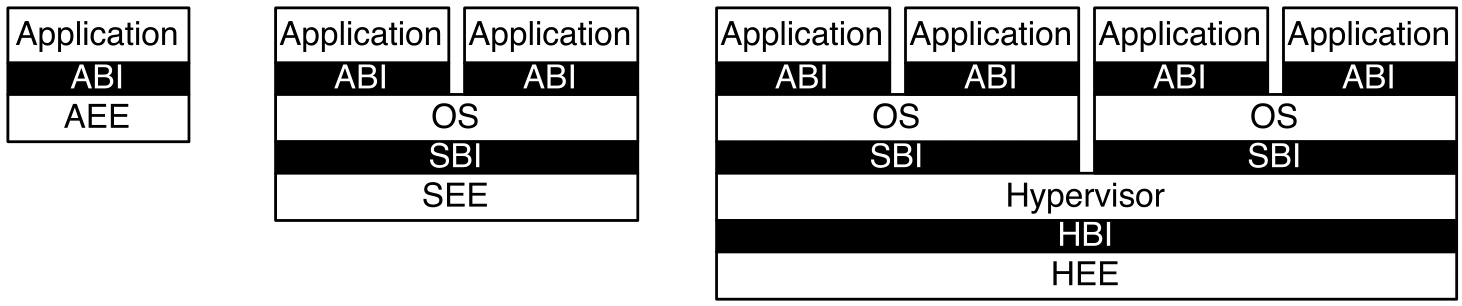
\includegraphics{figures/software-stacks.png}
%\caption{software-stacks}
%\end{figure}

上图中各个英文缩写对应的全称如下

\begin{itemize}
\item
  ABI: Application Binary Interface
\item
  AEE: Application Execution Environment
\item
  SBI: Supervisor Binary Interface
\item
  SEE: Supervisor Execution Environment
\item
  HBI: Hypervisor Binary Interface
\item
  HEE: Hypervisor Execution Environment
\end{itemize}

RISC-V通过各层之间的Binary
Interface实现了对下一层的抽象,方便了虚拟机的实现以及OS在不同RISC-V架构间的移植。采用了图中第二种结构,\href{https://github.com/riscv/riscv-pk}{bbl}在其中充当了SEE的角色。

\subsubsection{Privilege Levels}\label{privilege-levels}

RISC-V共有4种不同的特权级,与x86不同的是,RISC-V中特权级对应数字越小,权限越低

\begin{longtable}[c]{@{}cccc@{}}
\toprule
Level & Encoding & Name & Abbreviation\tabularnewline
\midrule
\endhead
0 & 00 & User/Application & U\tabularnewline
1 & 01 & Supervisor & S\tabularnewline
2 & 10 & Hypervisor & H\tabularnewline
3 & 11 & Machine & M\tabularnewline
\bottomrule
\end{longtable}

一个RISC-V的实现并不要求同时支持这四种特权级,可接受的特权级组合如下

\begin{longtable}[c]{@{}cll@{}}
\toprule
Number of levels & Supported Modes & Intended Usage\tabularnewline
\midrule
\endhead
1 & M & Simple embedded systems\tabularnewline
2 & M, U & Secure embedded systems\tabularnewline
3 & M, S, U & Systems running Unix-like operating systems\tabularnewline
4 & M, H, S, U & Systems running Type-1 hypervisors\tabularnewline
\bottomrule
\end{longtable}

目前官方的\href{https://github.com/riscv/riscv-isa-sim}{Spike}模拟器只部分实现了3个特权级。

\subsubsection{Control and Status
Registers}\label{control-and-status-registers}

RISC-V中各个特权级都有单独的Control and Status Registers
(CSRs),其中应当注意的有以下几个

\begin{longtable}[c]{@{}ll@{}}
\toprule
Name & Description\tabularnewline
\midrule
\endhead
sstatus & Supervisor status register\tabularnewline
sie & Supervisor interrupt-enable register\tabularnewline
stvec & Supervisor trap handler base address\tabularnewline
sscratch & Scratch register for supervisor trap handlers\tabularnewline
sepc & Supervisor exception program counter\tabularnewline
scause & Supervisor trap cause\tabularnewline
sbadaddr & Supervisor bad address\tabularnewline
sip & Supervisor interrupt pending\tabularnewline
sptbr & Page-table base register\tabularnewline
mstatus & Machine status register\tabularnewline
medeleg & Machine exception delegation register\tabularnewline
mideleg & Machine interrupt delegation register\tabularnewline
mie & Machine interrupt-enable register\tabularnewline
mtvec & Machine trap-handler base address\tabularnewline
mscratch & Scratch register for machine trap handlers\tabularnewline
mepc & Machine exception program counter\tabularnewline
mcause & Machine trap cause\tabularnewline
mbadaddr & Machine bad address\tabularnewline
mip & Machine interrupt pending\tabularnewline
\bottomrule
\end{longtable}

在继续阅读前,读者应当查阅\href{https://riscv.org/specifications/privileged-isa}{Privileged
Spec 1.9.1}以熟悉以上CSR的功能和用途。

\paragraph{CSR Instructions}\label{csr-instructions}

RISC-V
ISA中提供了一些修改CSR的原子操作,下面介绍之后常用到的\texttt{csrrw}指令

\begin{lstlisting}[language={C}]
# Atomic Read & Write Bit
cssrw rd, csr, rs
\end{lstlisting}

语义上等价的C++函数如下

\begin{lstlisting}[language={C}]
void cssrw(unsigned int& rd, unsigned int& csr, unsigned int& rs) {
   unsigned int tmp = rs;
   rd = csr;
   csr = tmp;
}
\end{lstlisting}

几种有趣的用法如下

\begin{lstlisting}[language={C}]
# csr = rs
cssrw x0, csr, rs

# csr = 0
cssrw x0, csr, x0

# rd = csr, csr = 0
cssrw rd, csr, x0

# swap rd and csr
cssrw rd, csr, rd
\end{lstlisting}


\section{“麻雀“OS--uCore}

为了学习OS,需要了解一个上百万代码的操作系统吗?自己写一个操作系统难吗?别被现在上百万行的Linux和Windows操作系统吓倒。当年Thompson乘他老婆带着小孩度假留他一人在家时,写了UNIX;当年Linus还是一个21岁大学生时完成了Linux雏形。站在这些巨人的肩膀上,我们能否也尝试一下做“巨人”的滋味呢?

MIT的Frans Kaashoek等在2006年参考PDP-11上的UNIX Version 6写了一个可在X86上跑的操作系统xv6(基于MIT License),用于学生学习操作系统。我们可以站在他们的肩膀上,基于xv6的设计,尝试着一步一步完成一个从“空空如也”到“五脏俱全”的“麻雀”操作系统—ucore,此“麻雀”包含虚存管理、进程管理、处理器调度、同步互斥、进程间通信、文件系统等主要内核功能,总的内核代码量(C+asm)不会超过5K行。充分体现了“小而全”的指导思想。

ucore的运行环境可以是真实的计算机系统,目前支持运行在X86,MIPS,ARM,RISC-V等计算机系统中。不过考虑到调试和开发的方便,我们可采用硬件模拟器,比如QEMU、BOCHS、VirtualBox、VMware Player等。ucore的开发环境主要是GCC中的gcc、gas、ld和MAKE等工具,也可采用集成了这些工具的IDE开发环境Eclipse-CDT。运行环境和开发环境既可以在Linux或Windows中使用。

那我们准备如何一步一步实现ucore呢?安装一个操作系统的开发过程,我们可以有如下的开发步骤:

\begin{enumerate}
	\def\labelenumi{\arabic{enumi}.}
	\item
	bootloader+toy
	ucore:理解操作系统启动前的硬件状态和要做的准备工作,了解运行操作系统的外设硬件支持,操作系统如何加载到内存中,理解两类中断--``外设中断'',``陷阱中断'',内核态和用户态的区别;
	\item
	物理内存管理:理解x86分段/分页模式,了解操作系统如何管理物理内存;
	\item
	虚拟内存管理:理解OS虚存的基本原理和目标,以及如何结合页表+中断处理(缺页故障处理)来实现虚存的目标,如何实现基于页的内存替换算法和替换过程;
	\item
	内核线程管理:理解内核线程创建、执行、切换和结束的动态管理过程,以及内核线程的运行周期等;
	\item
	用户进程管理:理解用户进程创建、执行、切换和结束的动态管理过程,以及在用户态通过系统调用得到内核中各种服务的过程;
	\item
	处理器调度:理解操作系统的调度过程和调度算法;
	\item
	同步互斥与进程间通信:理解同步互斥的具体实现以及对系统性能的影响,研究死锁产生的原因,如何避免死锁,以及线程/进程间如何进行信息交换和共享;
	\item
	文件系统:理解文件系统的具体实现,与进程管理和内存管理等的关系,缓存对操作系统IO访问的性能改进,虚拟文件系统(VFS)、buffer~cache和disk~driver之间的关系。
\end{enumerate}

其中每个开发步骤都是建立在上一个步骤之上的,就像搭积木,从一个一个小木块,最终搭出来一个小房子。在搭房子的过程中,完成从理解操作系统原理到实践操作系统设计与实现的探索过程。

%这个房子最终的建筑架构和建设进度如下图所示
%\textgreater{} (!可进一步标注处各个proj在下图中的位置)
%\begin{figure}[htbp]
%	\centering
%	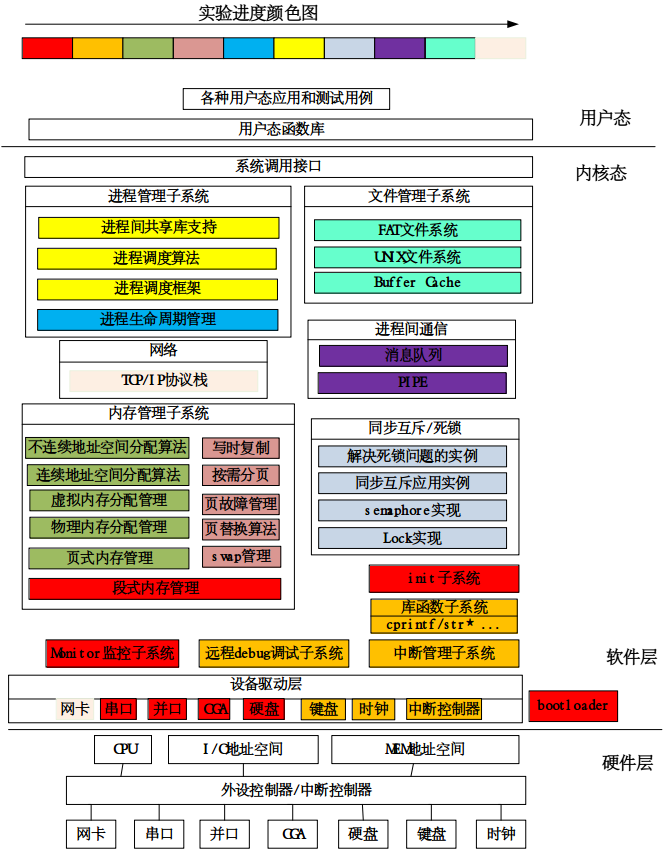
\includegraphics{figures/ucore_arch.png}
%	\caption{ucore操作系统架构}
%\end{figure}

\section{小结}
本章以分析一个“hello world”程序的执行过程为例子,概要地介绍了操作系统运行的计算机硬件架构,包括CPU、内存和外设,并对操作系统的历史发展、定义、目标、接口、抽象和特征等进行了阐述。最后简要介绍了课程实验用到的ucore操作系统。